\section{Consequences of the proof}\label{sec:consequences}
The results of this section are not needed for Theorem~\ref{thm:main}. They make the
construction quantitative and more flexible.

\subsection{The feedback deficit in closed form}
\begin{proposition}\label{prop:deficit}
For every \(n\ge2\), the stability margin \(1-G_n\) of the limiting prefix in
Lemma~\ref{lem:gain} is
\begin{equation}\label{eq:deficit}
 1-G_n=\frac{(3n-2)(50n-45)\,(2/9)^{n-1}}{9\,\bigl[14-8(3n-2)(2/9)^{n-1}\bigr]},
 \qquad 1-G_n\sim\frac{25}{21}\,n^2\Bigl(\frac29\Bigr)^{n-1}\quad(n\to\infty).
\end{equation}
\end{proposition}
\begin{proof}
Insert \(v=(3n-2)(2/9)^{n-1}\) from \eqref{eq:vmu} into \eqref{eq:gainfinal}; the asymptotic
statement follows from \(v\to0\) and \(3\cdot50/(9\cdot14)=25/21\).
\end{proof}

\begin{table}[ht]
\centering
\caption{The coefficient fraction \(v_n\) and the feedback deficit \(1-G_n\) of the limiting
prefix (exact values and decimal approximations).}\label{tab:deficit}
\begin{tabular}{cccccccc}
\toprule
\(n\) & 2 & 3 & 4 & 5 & 6 & 7 & 8\\
\midrule
\(v_n\) & \(\frac89\) & \(\frac{28}{81}\) & \(\frac{80}{729}\) & \(\frac{208}{6561}\) &
 \(\frac{512}{59049}\) & \(\frac{1216}{531441}\) & \(\frac{2816}{4782969}\)\\[4pt]
\(1-G_n\) & \(\frac{220}{279}\) & \(\frac{14}{39}\) & \(\frac{6200}{43047}\) &
 \(\frac{4264}{81171}\) & \(\frac{4352}{246777}\) & \(\frac{185440}{33437007}\) &
 \(\frac{499840}{301225671}\)\\[4pt]
decimal & \(0.789\) & \(0.359\) & \(0.144\) & \(0.0525\) & \(0.0176\) & \(0.00555\) & \(0.00166\)\\
\bottomrule
\end{tabular}
\end{table}

\begin{figure}[ht]
\centering
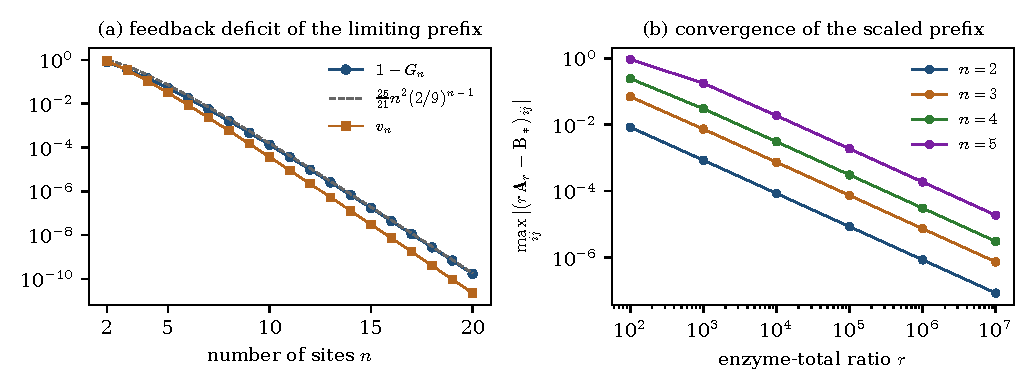
\includegraphics[width=\linewidth]{figures/deficit.pdf}
\caption{(a) The feedback deficit \eqref{eq:deficit}, its asymptote, and the coefficient
fraction \(v_n\). (b) The entrywise distance between \(r\bA_r\), computed exactly from the
coalesced construction, and its limit \(\bB_*\); the slope is \(-1\), in agreement with the
\(O(1/r)\) errors in Section~\ref{sec:prefix}.}\label{fig:deficit}
\end{figure}

The deficit is positive for every \(n\) but decays geometrically (Table~\ref{tab:deficit},
Figure~\ref{fig:deficit}(a)). This explains why the construction works for all \(n\) and is
nevertheless poorly conditioned for large \(n\). The decay is a property of this construction,
with all roots coalesced at \(x=3\) and \(A=(1+u)D\); it is not a lower bound on the time
scales or the resources that \(n\) stable states require.

\subsection{Diagonal stability and independent catalytic currents}
Lemma~\ref{lem:gain} used one vector of catalytic currents, \((1,\dots,1,t)\). A diagonal
Lyapunov matrix removes this restriction. Let \(\bz=\bH^{-1}\one\) and \(\bw=\bH^{-1}\bphi\);
both are entrywise positive.

\begin{proposition}[Diagonal Lyapunov matrix]\label{prop:diagonal}
Let \(\bP=\diag(w_i/z_i)\) and \(\bQ_*=\bB_*^{T}\bP+\bP\bB_*\). Then \(\bQ_*\) is negative
definite. Consequently, for all sufficiently large \(r\), \(\bA_r^{T}\bP+\bP\bA_r\) is negative
definite, and for every such \(r\) and every positive diagonal matrix \(\boldsymbol\Omega\) the
matrix \(\bA_r\boldsymbol\Omega\) is Hurwitz.
\end{proposition}
\begin{proof}
Since \(\bH\) is symmetric, \(\one^{T}\bw=\bz^{T}\bphi=G\). Hence \(\bB_*\bz=-(1-G)\one\) and
\(\bB_*^{T}\bw=-\bphi+G\bphi=-(1-G)\bphi\). Because \(\bP\bz=\bw\),
\[
 \bQ_*\bz=\bB_*^{T}\bw+\bP\bB_*\bz=-(1-G)\bigl(\bphi+\bP\one\bigr)<0 .
\]
The matrix \(\bQ_*\) is symmetric with nonnegative off-diagonal entries \(Q_{ik}\), because
\(\bB_*\) has nonnegative off-diagonal entries and \(\bP\) is a positive diagonal matrix. For
such a matrix and any positive vector \(\bz\), expanding the squares gives the identity
\begin{equation}\label{eq:energy}
 \boldsymbol a^{T}\bQ_*\boldsymbol a=\sum_i\frac{(\bQ_*\bz)_i}{z_i}\,a_i^2
 -\sum_{i<k}Q_{ik}\,z_iz_k\Bigl(\frac{a_i}{z_i}-\frac{a_k}{z_k}\Bigr)^2 ,
\end{equation}
which is negative for \(\boldsymbol a\ne0\). Negative definiteness is an open condition, and
\(r\bA_r\to\bB_*\). Finally
\((\bA_r\boldsymbol\Omega)^{T}(\boldsymbol\Omega\bP)+(\boldsymbol\Omega\bP)(\bA_r\boldsymbol\Omega)
=\boldsymbol\Omega(\bA_r^{T}\bP+\bP\bA_r)\boldsymbol\Omega\) is negative definite, and
\(\boldsymbol\Omega\bP\) is positive definite, so \(\bA_r\boldsymbol\Omega\) is Hurwitz by
Lyapunov's theorem.
\end{proof}

\begin{corollary}[Independent prefix currents]\label{cor:currents}
Let \(n\ge2\), let \(r\) be as in Proposition~\ref{prop:diagonal}, and let
\(\mathcal K\subset\R^{n-1}_{>0}\) be compact. There are \(t>0\), \(\varepsilon>0\) and
\(\delta_0>0\) such that the conclusions of Theorems~\ref{thm:main}\textup{(b)}
and~\ref{thm:split} hold for the construction of Section~\ref{sec:lift} with the catalytic
currents \((\omega_1,\dots,\omega_{n-1},t)\) at the coalesced equilibrium, for every
\((\omega_1,\dots,\omega_{n-1})\in\mathcal K\) and every \(0<\delta\le\delta_0\).
\end{corollary}
\begin{proof}
By Proposition~\ref{prop:diagonal} the prefix \(\bA_r\diag(\omega_1,\dots,\omega_{n-1})\) is
Hurwitz for every point of \(\mathcal K\), with a spectral bound that is uniform by
compactness. The arguments of Lemmas~\ref{lem:slowlink} and~\ref{lem:fullspectral} and of the
proof of Theorem~\ref{thm:split} use only the continuity of eigenvalues and the exact zero
provided by \eqref{eq:detzero} and Lemma~\ref{lem:Ksingular}. All matrices involved depend
continuously on the point of \(\mathcal K\), so \(t\), \(\varepsilon\) and \(\delta_0\) can be
chosen uniformly on \(\mathcal K\).
\end{proof}

The currents \(\omega_1,\dots,\omega_{n-1}\) are source-preserving coordinates; they are not
independent perturbations of the original rate constants, which are covered by
Theorem~\ref{thm:main}(c). No uniformity over unbounded sets of currents is claimed.

\subsection{Readout and the separation--recovery trade-off}
A natural observable is the total amount of fully phosphorylated substrate, \(S_n+Y_n\). At the
equilibrium of the construction of Section~\ref{sec:construction} with auxiliary coordinate
\(x\), formulas \eqref{eq:states} and \eqref{eq:sf} with \(t_n=D_{n-1}\) give
\begin{equation}\label{eq:readout}
 S_n+Y_n=\mathcal R(x):=\frac{D_{n-1}}{2}\cdot\frac{u^{n-1}}{D(u)}\cdot\frac{(x-1)(x+5)}{x+1},
 \qquad u=\frac{x^2-1}{8}.
\end{equation}
The function \(u^{n-1}/D(u)=1/\sum_iD_iu^{i-(n-1)}\) is nondecreasing, and
\((x-1)(x+5)/(x+1)=x+3-8/(x+1)\) has derivative \(1+8/(x+1)^2>0\). Hence \(\mathcal R\) is
strictly increasing: the readout orders the \(2n-1\) equilibria in the same way as the ratio
\(E/F\), and sinks and saddles alternate along it. Also \(E=(x-1)/2\) and \(F=4/(x+1)\) at these
equilibria, so the total phosphorylation flux \(\sum_i\gamma_iY_i\) is positive at each of
them; they are nonequilibrium steady states sustained by the irreversible catalytic steps.

\begin{corollary}\label{cor:tradeoff}
In the split family of Theorem~\ref{thm:split},
\[
 \mathcal R(x_j)-\mathcal R(x_k)=\mathcal R_\circ'(3)\,(\xi_j-\xi_k)\,\delta+O(\delta^2),\qquad
 \frac{1}{|\lambda_j(\delta)|}=\frac{1+O(\delta)}{a\,\prod_{k\ne j}|\xi_j-\xi_k|}\;\delta^{-(2n-2)},
\]
where \(\mathcal R_\circ\) is the function \eqref{eq:readout} of the coalesced system and
\(\mathcal R_\circ'(3)>0\).
\end{corollary}
\begin{proof}
At each \(\delta\) all equilibria share the polynomial \(D=D^{(\delta)}\), so the dependence of
\(D\) on \(\delta\) cancels from the difference to first order. The second formula is
\eqref{eq:splitlaw}.
\end{proof}

Thus, within this near-coalescence family, separating the states by an amount \(\delta\) costs
a linear relaxation time of order \(\delta^{-(2n-2)}\). This is a statement about the family,
not a speed limit for the network, and it suggests looking for well-separated roots when
designing examples; Section~\ref{sec:benchmark} does so.

\subsection{Labels, and a terminating design procedure}
\begin{corollary}\label{cor:labels}
A single sequential distributive cycle admits \(q\) simultaneously stable positive equilibria,
for one rate vector and one triple of totals, if and only if \(n\ge q\). In particular
\(2^{b}\) distinct stable equilibrium labels require \(n\ge2^{b}\) sites.
\end{corollary}
\begin{proof}
If \(n\ge q\), Theorem~\ref{thm:main}(b) gives \(n\ge q\) sinks; the converse is
Theorem~\ref{thm:main}(a).
\end{proof}

Coupled modules, transient codes and oscillatory phases are outside this statement, and it is
not a statement about an information rate in the presence of noise.

\begin{remark}[Exact design]\label{rem:design}
For fixed \(n\ge2\), fix strictly ordered rational offsets
\(\xi_0<\cdots<\xi_{2n-2}\) and use the candidates
\(r=2^a\), \(t=2^{-b}\), \(\varepsilon=2^{-c}\), and
\(\delta=2^{-d}\), with nonnegative integer indices, in the order
\eqref{eq:order}. A source candidate is eligible only when
\(r\ge3n/2\) and both coalesced converted polynomials \(B_{\raw}\)
and \(D_{\raw}\) have strictly positive coefficients through degree
\(n-1\) and no higher coefficients. Double \(r\) until an eligible
candidate passes the original exact Routh test for \(\bA_r\), or the
specified exact Lyapunov \(LDL^T\) test. Freeze the catalytic scales at
this positive coalesced state, giving unit prefix currents and final
current \(t\). Halve \(t\), starting at one, until the slow matrix has
a simple zero and a Hurwitz deflation; halve \(\varepsilon\), starting
at one, until the coalesced restricted Jacobian has the same property.
Finally halve \(\delta\), starting at one. A distance candidate is
eligible only when all prescribed roots \(x_j=3+\delta\xi_j\) exceed one
and its converted \(B_{\raw},D_{\raw}\) again satisfy the finite
coefficient conditions above. Stop at the first eligible candidate
whose original \(2n-1\) exact Routh tests give the alternating pattern.

All eligibility tests use finite rational arithmetic. Large-source
conversion positivity makes the first guard eventually true along the
doubling sequence. At each admitted source, continuity at coalescence
makes the last guard eventually true along the halving sequence. Thus
these guards do not obstruct eventual success of the corresponding
spectral tests. The positive coalesced state gives positive frozen
catalytic factors; \(t>0\) and \(0<\varepsilon\le1\) persist under all
later halvings. Every returned design therefore has positive rates and
the same prescribed positive equilibrium family at the common totals.
The termination argument uses the corresponding spectral lemmas and
the exact spectral tests' necessity and soundness. No bound on the
number of steps is claimed. Separately, Proposition~\ref{prop:witness}
certifies explicit rational systems for \(n\le7\); those systems are not
asserted to be outputs of this guarded asymptotic search.
\end{remark}

\section{Exact examples}\label{sec:examples}

\subsection{Rational witnesses for \texorpdfstring{\(n\le7\)}{n at most 7}}
The proof of Theorem~\ref{thm:main}(b) is asymptotic in \(r\), \(t\), \(\varepsilon\) and
\(\delta\). For small \(n\), direct rational tests give the explicit witnesses below
with moderate \(r\) and \(\delta\), unit coalesced currents and no binding relaxation.
They are certified at the displayed parameters; the sufficient large-source guard
in Remark~\ref{rem:design} is not required for this finite verification.

\begin{proposition}[Computer-assisted]\label{prop:witness}
Let \(2\le n\le7\), and let \((r,\delta)\) be \((2,\tfrac12)\), \((4,\tfrac12)\),
\((4,\tfrac12)\), \((8,\tfrac14)\), \((8,\tfrac14)\), \((8,\tfrac14)\) for \(n=2,\dots,7\). Let
\(x_j=3+\delta\,(j-n+1)\) for \(0\le j\le2n-2\), let the geometry be given by
\eqref{eq:normalize}, and let the kinetics be given by \eqref{eq:freedom} with
\(b_i=\beta_i=1\) and \(\theta_i=1/Y_i(X_\circ)\), where \(X_\circ\) is the coalesced
equilibrium \eqref{eq:coalstate} for the same \(r\); no relaxation \eqref{eq:relaxation} is
applied. Then the system with totals \((2r,2,2r+2)\) has exactly \(2n-1\) positive equilibria;
the \(n\) equilibria with even index are sinks, and at each of the \(n-1\) equilibria with odd
index exactly one eigenvalue of \(\JS\) has positive real part and none lies on the imaginary
axis.
\end{proposition}
\begin{proof}
For each of the \(48\) equilibria the rational matrix \(\JS\) was formed, its characteristic
polynomial was computed exactly by the Faddeev--LeVerrier recursion in integer arithmetic, with
the Cayley--Hamilton identity as a check, and the Routh array \cite[Ch.~XV]{Gantmacher} was
formed in rational arithmetic. In every case all \(3n+1\) entries of the first column are
nonzero, and the number of sign changes is \(0\) for even \(j\) and \(1\) for odd \(j\). The
count of equilibria is Theorem~\ref{thm:count}.
\end{proof}

\begin{example}[Two sites]\label{ex:two}
For \(n=2\), \(r=2\) and \(x=(\tfrac52,3,\tfrac72)\) one finds \(N=\tfrac{111}{4}+8u\),
\(J=\tfrac{15}{4}+32u\), \(D=1+\tfrac{8672}{2625}u\), \(B=\tfrac{1287}{125}+\tfrac{2288}{875}u\),
the totals \((\ET,\FT,\ST)=(4,2,6)\), and the rate constants
\[
\begin{array}{c|cccccc}
 i & a_i & b_i & c_i & \alpha_i & \beta_i & \gamma_i\\\hline
 1 & \tfrac{19782}{1375} & 1 & \tfrac{625}{1573} & \tfrac{147000}{124267} & 1 & \tfrac{45}{11}\\[3pt]
 2 & \tfrac{311808}{192049} & 1 & \tfrac{4065}{2431} & \tfrac{79}{34} & 1 & \tfrac{45}{34}
\end{array}
\]
The three equilibria, in the order \((S_0,S_1,S_2;\,E,F;\,C_1,C_2;\,Y_1,Y_2)\), are
\begin{align*}
 X_0&=\bigl(\tfrac{250}{693},\tfrac{1027}{1008},\tfrac{271}{528};\ \tfrac34,\tfrac87;\
 \tfrac{39}{14},\tfrac{13}{28};\ \tfrac{125}{462},\tfrac{271}{462}\bigr),\\
 X_1&=\bigl(\tfrac{2625}{11297},1,\tfrac{8672}{11297};\ 1,1;\
 \tfrac{189}{79},\tfrac{48}{79};\ \tfrac{2625}{11297},\tfrac{8672}{11297}\bigr),\\
 X_2&=\bigl(\tfrac{350}{2223},\tfrac{869}{912},\tfrac{4065}{3952};\ \tfrac54,\tfrac89;\
 \tfrac{77}{38},\tfrac{55}{76};\ \tfrac{875}{4446},\tfrac{1355}{1482}\bigr).
\end{align*}
\(X_0\) and \(X_2\) are sinks and \(X_1\) is a saddle. The eigenvalues of largest real part,
computed in floating point, are approximately \(-0.0120\), \(+0.0050\) and \(-0.0084\); the
remaining ones have real parts below \(-2\).
\end{example}

\subsection{A three-site benchmark with separated states}\label{sec:benchmark}
The witnesses above are close to coalescence. For a benchmark with well-separated states we
take \(n=3\),
\[
 x=(2,\tfrac72,5,\tfrac{13}{2},8),\qquad r=9,\qquad (\ET,\FT,\ST)=(18,2,20),
\]
for which \(N=\tfrac{10165}{4}+1926u+64u^2\), \(J=\tfrac{385}{2}+3562u+768u^2\) and
\[
 D=1+\tfrac{505005048}{38591245}u+\tfrac{48362752}{38591245}u^2,\qquad
 B=\tfrac{111414528}{1102607}+\tfrac{5946508756}{38591245}u+\tfrac{236379904}{38591245}u^2 .
\]
The nine kinetic parameters \((\theta_i,b_i,\beta_i)\) were chosen by a bounded numerical
search that maximizes the smallest decay rate at the three even-indexed equilibria, subject to
the ceilings \(a_i,\alpha_i\le2\) and \(b_i,c_i,\beta_i,\gamma_i\le2\) in model units; the
ceilings remove the trivial improvement obtained by rescaling time. The result was rounded to
rational numbers, and everything stated below refers to these exact rational rate constants,
which are distributed with the source. Three root geometries were compared in this way; the
smallest decay rates found were \(0.80\times10^{-4}\), \(0.98\times10^{-4}\) and
\(1.26\times10^{-4}\) for \(x=(2,3,4,5,6)\), \((\tfrac32,\tfrac52,\tfrac72,\tfrac92,\tfrac{11}2)\) and
the geometry selected here. These numbers are floating-point diagnostics, and the search makes
no claim of optimality.

\begin{proposition}[Computer-assisted]\label{prop:benchmark}
For the benchmark rate constants the class with totals \((18,2,20)\) contains exactly five
positive equilibria, listed in Table~\ref{tab:states}. The equilibria \(X_0,X_2,X_4\) are
sinks, and \(X_1,X_3\) are hyperbolic saddles with one unstable direction.
\end{proposition}
\begin{proof}
The rate constants realize the geometry above through \eqref{eq:freedom}, so
Theorem~\ref{thm:count} applies (\(r=9>\max_ju_j=\tfrac{63}{8}\) and
\(4r+\sqrt{1+8r}>36>25=\sum_jx_j\)). The stability statements are exact Routh computations as
in Proposition~\ref{prop:witness}.
\end{proof}

\begin{table}[ht]
\centering
\caption{The five equilibria of the three-site benchmark. Concentrations in the last two
columns are in \(\mu\)M for the unit \(C_0=0.1\,\mu\)M; decimal entries are rounded values of
exact rational numbers. ``Unstable'' is the number of eigenvalues of \(\JS\) in the open right
half-plane, from an exact Routh array.}\label{tab:states}
\begin{tabular}{cccccccc}
\toprule
\(j\) & \(x_j\) & \(u=E/F\) & \(E\) & \(F\) & \(\Phi'(u_j)\) & \(S_3+Y_3\) (\(\mu\)M) & unstable\\
\midrule
0 & \(2\) & \(3/8\) & \(1/2\) & \(4/3\) & \(-0.29235\) & \(0.003380\) & 0\\
1 & \(7/2\) & \(45/32\) & \(5/4\) & \(8/9\) & \(\phantom{-}0.02050\) & \(0.026743\) & 1\\
2 & \(5\) & \(3\) & \(2\) & \(2/3\) & \(-0.00772\) & \(0.072950\) & 0\\
3 & \(13/2\) & \(165/32\) & \(11/4\) & \(8/15\) & \(\phantom{-}0.01002\) & \(0.138019\) & 1\\
4 & \(8\) & \(63/8\) & \(7/2\) & \(4/9\) & \(-0.08439\) & \(0.216157\) & 0\\
\bottomrule
\end{tabular}
\end{table}

\begin{figure}[ht]
\centering
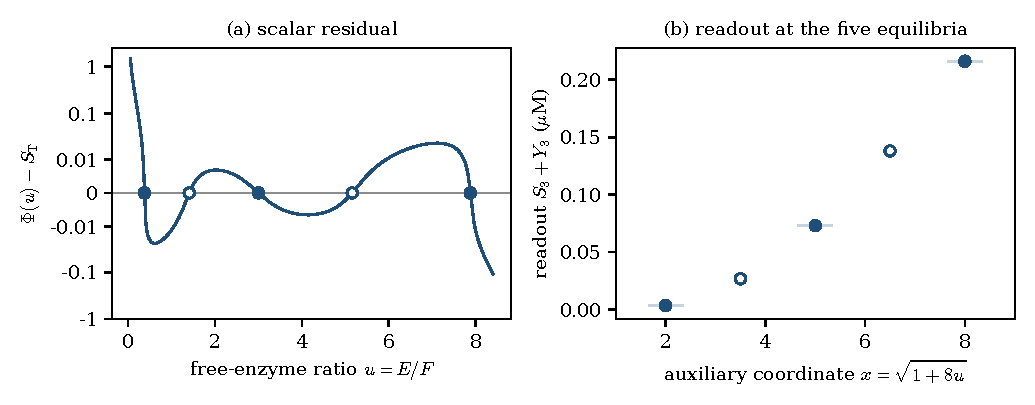
\includegraphics[width=\linewidth]{figures/benchmark.pdf}
\caption{The three-site benchmark. (a) The residual \(\Phi(u)-\ST\) on an
\(\operatorname{arcsinh}\) scale; filled markers are sinks, open markers are saddles. (b) The
readout \(S_3+Y_3\) at the five equilibria; the shaded bars are the certified readout intervals
of Proposition~\ref{prop:certificate}, including a measurement error of \(\pm0.001\,\mu\)M. The
curves and markers are drawn from exact rational data; the counts are certified by the
formulas and the Routh arrays, not by the plot.}\label{fig:benchmark}
\end{figure}

\paragraph{Declared units.}
To read the benchmark in physical units we declare a concentration unit \(C_0=0.1\,\mu\)M and a
time unit \(T_0=10\) s. Bimolecular constants are divided by \(C_0T_0\) and unimolecular
constants by \(T_0\). The totals become \((\ET,\FT,\ST)=(1.8,\,0.2,\,2.0)\,\mu\)M, and the rate
constants are those of Table~\ref{tab:rates}. The association constants are at most
\(2\,\mu\mathrm M^{-1}\mathrm s^{-1}\) and the unimolecular constants at most
\(0.2\,\mathrm s^{-1}\). The slowest of the three numerically computed decay rates corresponds
to an e-folding time of about \(22\) hours. These units are declarations, not fits: the
unimolecular constants span a factor of about \(33{,}446\), the kinase total is comparable to
the substrate total, and no measured kinetic data were used. The benchmark is a reproducible
test case, not a model of a particular kinase--phosphatase pair.

\begin{table}[ht]
\centering
\caption{Rate constants of the three-site benchmark in the declared units, rounded to six
significant digits. The exact rational values in model units are distributed with the
source and are authoritative.}\label{tab:rates}
\begin{tabular}{ccccccc}
\toprule
Site & \(a_i\) (\(\mu\mathrm M^{-1}\mathrm s^{-1}\)) & \(b_i\) (\(\mathrm s^{-1}\)) &
\(c_i\) (\(\mathrm s^{-1}\)) & \(\alpha_i\) (\(\mu\mathrm M^{-1}\mathrm s^{-1}\)) &
\(\beta_i\) (\(\mathrm s^{-1}\)) & \(\gamma_i\) (\(\mathrm s^{-1}\))\\
\midrule
1 & \(2.00000\) & \(5.96184\times10^{-6}\) & \(0.00197333\) & \(0.171890\) & \(0.0427272\) & \(0.199398\)\\
2 & \(1.86875\) & \(7.83183\times10^{-4}\) & \(0.0162999\) & \(1.99626\) & \(0.0268102\) & \(0.191934\)\\
3 & \(0.217843\) & \(0.0126769\) & \(0.0383203\) & \(2.00000\) & \(0.0127038\) & \(0.187296\)\\
\bottomrule
\end{tabular}
\end{table}

\subsection{A rigorous local certificate for independent parameter errors}
Theorem~\ref{thm:main}(c) gives an open set of parameters without an estimate of its size. For
the benchmark we certify an explicit, if very small, neighbourhood, in which all \(18\) rate
constants and all three totals vary independently; in particular the perturbed systems need
not lie in the source-preserving family \eqref{eq:freedom}, and their equilibria move.

The certificate uses the exact model-unit parameters and concentrations; its times and
readouts are converted to the declared physical units by \(T_0\) and \(C_0\), respectively.
Let \(q=(S_1,S_2,S_3,C_1,C_2,C_3,Y_1,Y_2,Y_3)\) be the model-unit coordinates on the class, let \(q_0\) be
one of the three nominal sinks, and use the weighted deviations
\(e=\diag(q_0)^{-1}(q-q_\theta)\) from the equilibrium \(q_\theta\) of a perturbed parameter
vector \(\theta\). Let \(\JS_0\) be the restricted Jacobian in model time at \(q_0\) in the weighted
coordinates.

\begin{proposition}[Computer-assisted]\label{prop:certificate}
Let \(\epsilon_{\mathrm{rel}}=1/671088640000\approx1.49\times10^{-12}\), and let each of the
\(18\) rate constants and the three totals of the benchmark vary independently within the
relative distance \(\epsilon_{\mathrm{rel}}\) of its nominal value. For each of the three
nominal sinks \(X_0,X_2,X_4\), with the radii \(\varrho_0\) and \(\varrho_{\mathrm{in}}\) of
Table~\ref{tab:certificate}:
\begin{enumerate}
\item[\textup{(i)}] the perturbed system has exactly one equilibrium \(q_\theta\) in the box
\(\|\diag(q_0)^{-1}(q-q_0)\|_\infty\le\varrho_0\); it is positive and satisfies
\(\|\diag(q_0)^{-1}(q_\theta-q_0)\|_\infty\le\varrho_0/4\);
\item[\textup{(ii)}] there is a rational symmetric positive definite matrix \(\bP\), the same
for all admitted parameters, such that every solution with \(\|e(0)\|_2\le\varrho_{\mathrm{in}}\)
stays in that box and satisfies
\[
 \|e(t)\|_2\le\frac{\varrho_0}{2}\,\exp\Bigl(-\frac{c}{2M}\,\frac{t}{T_0}\Bigr),
 \qquad M=\|\bP\|_\infty,\quad c=\frac{1}{\|\bQ^{-1}\|_\infty}-\ell_{\mathrm{loss}}>0,
\]
where \(\bQ=-(\JS_0^{T}\bP+\bP\JS_0)\) and \(\ell_{\mathrm{loss}}\) is an interval bound for the
variation of \(\JS^{T}\bP+\bP\JS\) over the box and over all admitted parameters; in particular
\(\|e(t)\|_2\) has decreased below \(\varrho_0/20\) after the time \(T_{10}=60M/c\) seconds of
Table~\ref{tab:certificate};
\item[\textup{(iii)}] the readouts \(S_3+Y_3\) at the three perturbed sinks, with a measurement
error of \(\pm0.001\,\mu\mathrm M\) added, lie in the pairwise disjoint intervals
\([0.00237970,0.00437971]\), \([0.07195005,0.07395006]\) and
\([0.21515666,0.21715672]\) (\(\mu\)M).
\end{enumerate}
\end{proposition}
\begin{proof}
All steps are carried out in rational or rational-interval arithmetic. A floating-point
Lyapunov solve proposes \(\bP\), which is then rounded to a rational matrix; exact \(LDL^{T}\)
factorizations verify that \(\bP\) and \(\bQ\) are positive definite. Since \(\bP\) and
\(\bQ^{-1}\) are symmetric, their spectral norms are at most their \(\infty\)-norms, so
\(\bP\preceq M\bI\) and \(\bQ\succeq\|\bQ^{-1}\|_\infty^{-1}\bI\).

(i) For the Newton-type map \(q\mapsto q-\JS_0^{-1}g_\theta(q)\) (in weighted coordinates),
interval evaluation over the box and the parameter set shows that its derivative has
\(\infty\)-norm at most some \(\vartheta\le\tfrac12\) and that it moves \(q_0\) by at most
\((1-\vartheta)\varrho_0/4\); by the contraction principle it has a unique fixed point in the
box, within \(\varrho_0/4\) of \(q_0\), and the fixed points of this map in the box are exactly
the equilibria there. The same interval evaluation bounds all twelve concentrations away from zero. Here it
matters that each reaction vector is multiplied by \(\JS_0^{-1}\) (and, below, by \(\bP\))
\emph{before} the interval evaluation: this keeps the exact cancellations between the
reactions and improves the admissible \(\epsilon_{\mathrm{rel}}\) by about eight orders of
magnitude over a product of separate norm bounds.

(ii) For admitted \(\theta\) and \(q\) in the box, the segment from \(q_\theta\) to \(q\) lies in
the box, and the mean-value form of the vector field gives
\(\dot e=\bar\JS e\), where \(\bar\JS\) is an average of restricted Jacobians over the segment. The
interval bound gives
\(\|(\bar\JS-\JS_0)^{T}\bP+\bP(\bar\JS-\JS_0)\|_2\le\ell_{\mathrm{loss}}\), so for
\(V=e^{T}\bP e\),
\[
 \dot V\le-\bigl(\|\bQ^{-1}\|_\infty^{-1}-\ell_{\mathrm{loss}}\bigr)\|e\|_2^2=-c\,\|e\|_2^2
 \le-\frac cM\,V .
\]
Let \(p_{\min}\) be a rational lower bound for the smallest eigenvalue of \(\bP\). The
ellipsoid \(V\le p_{\min}(\varrho_0/2)^2\) lies in the Euclidean ball of radius \(\varrho_0/2\)
around \(q_\theta\), hence in the box, because the centre has moved by at most
\(\varrho_0/4\) in the \(\infty\)-norm; it is invariant; and it contains the ball
\(\|e\|_2\le\varrho_{\mathrm{in}}:=(\varrho_0/2)\sqrt{p_{\min}/M}\) (rounded down). On it,
\(\|e(t)\|_2^2\le V(t)/p_{\min}\le(\varrho_0/2)^2\exp(-ct/M)\) in model time. Since
\(\log10<3\), a tenfold decrease of this envelope is reached by the model time \(6M/c\), that
is, by \(60M/c\) seconds.

(iii) The readout is a linear function of \(q\), and (i) bounds the displacement of each sink.
\end{proof}

\begin{table}[ht]
\centering
\caption{The local certificate of Proposition~\ref{prop:certificate}. The column ``earlier''
is the bound obtained when the norms are rounded to powers of ten and half of the Lyapunov
margin is discarded; the column \(T_{10}\) keeps the exact constants. Times are rounded
upwards.}\label{tab:certificate}
\begin{tabular}{ccccccc}
\toprule
Sink & \(\varrho_0\) & \(\varrho_{\mathrm{in}}\) & \(M\) & \(c\) & \(T_{10}\) (s) & earlier (s)\\
\midrule
\(X_0\) & \(1/8192000\) & \(1/16384000000\) & \(5846.11\) & \(0.98516\) & \(357{,}000\) & \(1.2\times10^{7}\)\\
\(X_2\) & \(1/16384000\) & \(1/327680000000\) & \(535109.89\) & \(0.97537\) & \(32{,}918{,}000\) & \(1.2\times10^{9}\)\\
\(X_4\) & \(1/2048000\) & \(1/40960000000\) & \(383168.49\) & \(0.98112\) & \(23{,}433{,}000\) & \(1.2\times10^{9}\)\\
\bottomrule
\end{tabular}
\end{table}

The certificate should be read for what it is. The parameter tolerance
\(\epsilon_{\mathrm{rel}}\approx1.5\times10^{-12}\) and the neighbourhoods
\(\varrho_{\mathrm{in}}\) are far too small to represent laboratory tolerances, and the times
\(T_{10}\) are upper bounds for an envelope inside an invariant ellipsoid, not predicted
recovery times: the worst bound is about \(381\) days, whereas the numerically computed slowest
e-folding time is about \(22\) hours. Much of the gap between the two reflects the conditioning of
\(\bP\) (\(M\approx5\times10^5\)) rather than the dynamics. Keeping the exact rational
constants instead of rounded ones improved the worst bound \(36\)-fold, from about \(38\)
years, without changing the system, the parameter box or the neighbourhoods. What the
proposition does establish is that a full-dimensional, explicitly described set of parameters
supports three distinguishable, locally attracting states with quantified return.

\section{Formal verification and reproducibility}\label{sec:formal}
The development in Lean~4 \cite{Lean4} with Mathlib \cite{Mathlib} has an original
equilibrium-count part and an extended stable-capacity part. The original proofs use Lean
\texttt{v4.30.0}; this version selects nineteen independent statements under the Palomar
target Lean \texttt{v4.35.0-rc2}. The selected proof sources and required supporting modules
have compiled with warnings treated as errors.
The selected proof declarations contain no \texttt{sorry}; the permitted axiom list is
\texttt{propext}, \texttt{Classical.choice} and \texttt{Quot.sound}.
The independent Challenge states the claims using the literal model
and Mathlib definitions; its protocol statement placeholders are excluded from the proof
dependency closure. The source manifest and verification receipt identify the checked
snapshot separately from earlier release receipts. Independent checking uses the
Comparator and the con-ron, nanoda and Lean default kernels.

\emph{The equilibrium count.} The modules \texttt{Recurrence}, \texttt{Conversion},
\texttt{Source}, \texttt{Assembly} and \texttt{Resolution} of the namespace
\texttt{PhosphorylationSharpness} define the state space, the six rate constants per site, the
mass-action vector field of \eqref{eq:network} componentwise, and the three totals, and prove
\begin{quote}
\texttt{theorem sharp\_lower\_bound (n :\ $\mathbb N$) (hn :\ 1 $\le$ n) :\ Attains n (2*n-1)}
\end{quote}
where \texttt{Attains n k} states that there exist positive rate constants, positive totals and
an injective family of \(k\) positive states at which every component of the vector field
vanishes and the three totals take the given values. The statement contains no reduced
equation and no numerical input. The proof follows Section~\ref{sec:construction} for the roots
\(x_j=j+2\), except that positivity of \(D_{\raw}\) and \(B_{\raw}\) is proved for all
sufficiently large \(r\) by an elementary estimate based on \eqref{eq:qformula} instead of
Theorem~\ref{thm:positivity}. A further module, \texttt{PublicationAlgebra}, verifies
\eqref{eq:product} and coefficient positivity for arbitrary lists of roots greater than one,
the determinant \eqref{eq:pivot}, the factorization \eqref{eq:residual}, and the sign of the
prefactor in \eqref{eq:slope}.
The selected universal equilibrium-count theorem proves that, for arbitrary positive
rates and totals, the positive equilibrium set is finite and has cardinality at most
\(2n-1\). It applies independently of hyperbolicity.

\emph{The exact stable-state capacity and simultaneous attainment.} The extended namespace
\texttt{PhosphorylationStableCapacity} defines the literal \(3n\)-dimensional
compatibility-class field and a nonlinear stability predicate: every nearby initial state
admits a forward solution, all forward solutions remain nearby, and all forward solutions
from a neighborhood converge to the equilibrium. The selected capacity theorem is
\begin{quote}
\texttt{all\_size\_exact\_capacity\_with\_hyperbolic\_attainment\_435 :}\par
\texttt{\(\forall\) n, 1 \(\le\) n \(\to\)}\par
\texttt{ExactCapacityWithHyperbolicAttainment n}
\end{quote}
It combines attainment of \(n\) positive locally asymptotically stable equilibria with
Hurwitz class Jacobians for one common rate list and totals, and a universal bound of
\(n\) for every positive class.
The statement explicitly includes finiteness of the stable-state set as well as its
cardinality bound. The ceiling includes singular and nonhyperbolic local attractors.
The proof builds the
Hurwitz-to-nonlinear-stability transfer, an exact positive-equilibrium/scalar-root bijection,
regular-root signed counts and local indices of attracting states. Its topological input is
a closed-ball degree with boundary homotopy invariance, normalization and regular-zero
determinant formula; these laws are proved from a pinned finite-dimensional homological
degree development~\cite{LeanDifferentialGeometry} and transported to the actual
product-coordinate balls. The selected full-family theorems retain one common rate
vector and total triple for all \(2n-1\) equilibria. Their even-indexed \(n\)
members have Hurwitz class Jacobians and are nonlinear local attractors; each
odd-indexed member has exactly one eigenvalue with positive real part and all
remaining eigenvalues with negative real part. The full positive equilibrium set
equals this family. The selected rational theorem constructs such a system with
rational rates, totals, and equilibria for every \(n\ge1\). The selected openness
theorem supplies a nonempty open set in the full rate-and-total parameter space:
every parameter in the set has exactly this sink--saddle configuration, and the
set contains a rational attaining parameter.

\emph{Scope of the formal statements.} The nineteen selected statements retain the
all-size conclusions of Theorem~\ref{thm:main}(a)--(c): exact nonlinear stable-state
capacity, the universal positive-equilibrium ceiling, rational simultaneous attainment,
and persistence of the complete configuration on a nonempty open set of all rates and
totals. The stable-state ceiling includes singular and nonhyperbolic local attractors.
The attaining rational system has exactly \(2n-1\) positive equilibria for one common
rate vector and total triple: \(n\) nonlinear Hurwitz sinks and \(n-1\) hyperbolic saddles.
For each saddle the restricted Jacobian has one simple positive real eigenvalue, and every
other eigenvalue lies strictly in the left half-plane. Supporting Lean proofs construct
an analytic local unstable curve at every such positive saddle from the actual mass-action
field and this spectral condition. The curve is embedded and immersed, is tangent at the
equilibrium to its positive real eigenvector, and satisfies the field-invariance identity.
Its explicitly constructed backward trajectories stay on the curve and converge to the
equilibrium. Shrinking only the radius keeps the curve and these trajectories positive
and in the original compatibility class. A common-family theorem applies this construction
to every odd-index saddle of the same rational attaining system, while retaining its rates,
totals, complete equilibrium list, sink and saddle assertions, and exact count.
These are supporting formal results additional to the nineteen selected statements.

The selected arbitrary-source statement proves Lemmas~\ref{lem:interlace}
and~\ref{lem:ratios} for the actual recurrence whenever every prescribed root exceeds one,
including repeated prescribed roots and the degree-zero case. It gives complete simple
negative root lists for \(N,J\), their strict interlacing, both partial-fraction identities
off the respective poles, and strictly positive residues equal to the stated derivative
quotients. It also proves strict increase of \(J_{i-1}/J_i\), with \(J_{-1}=0\), and
nondecrease of \(J_i/N_i\). Separate selected coefficient statements prove positivity of
the actual conversion quotient and \(D_{\raw}\) for every \(r>0\), and positivity of
\(B_{\raw}\) under the literal hypotheses of Theorem~\ref{thm:positivity}(ii), including
the non-strict sum boundary. The selected readout statement proves strict monotonicity of
the physical scalar formula on all \(x>1\) for every dense positive \(D\).

The supporting prescribed-root construction retains the universal quantifiers of
Theorem~\ref{thm:count}: every strictly ordered real root list above one, every admissible
\(r\), and every choice of positive \((b_i,\beta_i,\gamma_i)\). It reconstructs the actual
normalized coefficient family and the rates of \eqref{eq:ratesgeneral}, proves positivity
of those rates, and retains the prescribed positive equilibrium list at the common totals
\((2r,2,2r+2)\), its exhaustion and exact count, and rational rates and concentrations
when the input data are rational. All listed equilibria are nondegenerate; the restricted
Jacobian at each odd index has an odd number of positive real eigenvalues, counted with
algebraic multiplicity. The same complete nondegenerate configuration persists on a
nonempty open neighborhood in the full positive rate-and-total parameter space.
This general kinetic construction is additional to the selected existential
stable-capacity attaining family.

For the quantitative splitting law, the selected statements retain the literal
fixed-binding family, its prescribed ordered offsets, common rates and totals, exhaustive
positive equilibrium list, analytic slow eigenvalues, and the normalized physical
coefficient in Theorem~\ref{thm:split}. The relative error and reciprocal relaxation bounds
use those same witnesses. Rational attainment is a rational member of that same law family.
The compact-current statements retain common construction parameters and uniform bounds
over arbitrary compact sets of positive prefix currents, including the empty set, and
throughout one common closed positive splitting interval. The interval statement also
retains positive readout derivative and positive total catalytic flux.

The selected finite statements classify all \(48\) printed equilibria for \(n=2,\ldots,7\),
prove the full five-equilibrium nominal three-site benchmark, and identify the printed
two-site dominant root and its five-root tail to the left of \(-2\). The operational
statement for Proposition~\ref{prop:certificate} permits independent relative changes of
all \(21\) physical inputs and retains the same three distinct equilibria, their positivity,
local uniqueness, hyperbolicity, fixed rational Lyapunov data, and every-solution recovery
from the printed inner balls and closed ellipsoids, including their boundaries. Its measured
readout extension keeps these same parameters and equilibria and proves strict ordering
under independently chosen errors of magnitude at most \(0.001\,\mu\mathrm M\).

Supporting checked modules formalize the original four nested first-success loops of
Remark~\ref{rem:design}, with their finite rational eligibility guards and the original
exact Routh tests. Necessity and soundness of the neutral, even and odd tests are proved
from the actual characteristic polynomials. Termination returns the same earliest
indices \(a,b,c,d\) with positive rational rates and states, common totals, equilibrium
exhaustion, the exact count, catalytic-current identities, nonlinear Hurwitz sinks and
one-unstable saddles. No bound on the number of steps is asserted. The independently
certified printed systems of Proposition~\ref{prop:witness} are not asserted to be the
search outputs. Exact Lyapunov and Euler certificate searches remain additional
constructive routes. Supporting modules also prove the closed feedback-deficit formula
and its asymptotic constant, the stable-label criterion, the limiting prefix block's
Hurwitz property for every positive current vector, and the readout and reciprocal-time
analytical corollaries using the same construction and eigenvalue witnesses.

{\sloppy\emph{Reproduction.} The source package contains the Lean modules, the exact data of
the benchmark, and a Python script, \texttt{check\_paper.py}, which uses only the standard
library and rational arithmetic. It verifies the construction for \(n\le6\) (equilibrium
equations, totals, the identity \eqref{eq:freeinventory}) for distinct and for coalesced roots;
Lemma~\ref{lem:interlace} by Sturm sequences, Lemma~\ref{lem:ratios}, and
Theorem~\ref{thm:positivity} at the boundary of its range, on random root configurations with
and without repeated roots; the moments \eqref{eq:moments} and \eqref{eq:vmu}, the positivity
of \(\bphi\), the gain formula \eqref{eq:gainfinal}, Table~\ref{tab:deficit}, and the
definiteness of \(\bQ_*\), for \(n\le8\); the exact identities of Lemma~\ref{lem:compression},
the singularity of \(\bK\), and the \(O(1/r)\) convergence \(r\bA_r\to\bB_*\) for \(n\le5\); the
determinant formula \eqref{eq:det} and the readout formula \eqref{eq:readout}; the base case
\(n=1\); Proposition~\ref{prop:witness} (for \(n\le4\) by default and for \(n\le7\) with the
option \texttt{-{}-full}); Example~\ref{ex:two}; and every number in
Section~\ref{sec:benchmark}, including an independent replay of the interval bounds of
Proposition~\ref{prop:certificate}. These computations test the exposition and the
implementation. The proofs of Theorems~\ref{thm:main} and~\ref{thm:split} do not depend on
them.\par}

\section{Discussion}\label{sec:discussion}
The sequential distributive \(n\)-site cycle has equilibrium capacity \(2n-1\) and stable-state
capacity \(n\), for every \(n\). Both values are attained by one explicit rational system, and
the stable ceiling holds without any nondegeneracy assumption. The reusable idea in the proof
is the separation of geometry and kinetics: the equilibrium equations see only half of the
parameters, so one can first build the richest possible equilibrium set, then coalesce it, and
then use the remaining parameters to organize time scales so that the transverse spectrum
becomes computable. In the present case the computation ends in a scalar gain with a closed
form.

We close with limitations and open questions.

\emph{Conditioning.} The proof is an existence proof with ordered limits. The margin
\eqref{eq:deficit} decays like \(n^2(2/9)^n\), the splitting law \eqref{eq:splitlaw} shows that
near coalescence the slowest rate is of order \(\delta^{2n-2}\), and the open set of
Theorem~\ref{thm:main}(c) comes without a size. Proposition~\ref{prop:witness} and the
benchmark show that for small \(n\) much better constants are available than the proof
suggests. It would be interesting to find a construction of \(n\) sinks whose spectral gap and
parameter tolerance decay at most polynomially in \(n\), or to show that none exists.

\emph{Enzyme levels.} In our examples \(\ST=\ET+\FT\) and the kinase is in large excess over
the phosphatase, so that most of the substrate is bound to the kinase; this is far from the
substrate-excess regime of Michaelis--Menten reductions, in which generically at most \(n+1\)
equilibria exist \cite[Theorem~4]{WangSontag2008}. How small \(\ET/\ST\) and \(\FT/\ST\) can be
in a system with \(2n-1\) equilibria, or with \(n\) sinks, is open. By the symmetry
\(E\leftrightarrow F\), \(S_i\leftrightarrow S_{n-i}\) of \eqref{eq:network} all results hold
with the roles of the enzymes exchanged.

\emph{Global dynamics.} Theorem~\ref{thm:main} bounds the number of attracting equilibria, not
the number of attractors. For \(n=1\) every trajectory converges to the unique equilibrium
\cite{AngeliSontag2008}. Whether the two-site cycle admits periodic orbits is a
well-known open question; see \cite{CMS2019,CFM2020,ConradiMincheva2024} for partial results
and related mechanisms. Our ceiling neither uses nor implies the absence of oscillations for
any \(n\), and attracting periodic orbits, if present, are not counted by \(\capC\). We do not
know the basins of the \(n\) sinks constructed here, and we do
not claim that they attract almost all initial conditions.

\emph{Thermodynamics and noise.} The catalytic steps in \eqref{eq:network} are irreversible
effective reactions. The constructed states carry a positive phosphorylation flux and
therefore presuppose a maintained chemical driving force; a closed system with a finite supply
of ATP cannot hold them indefinitely. A model with explicit fuel, or with reversible catalytic
steps, is a different network and requires its own analysis. Likewise, the theorem concerns
the deterministic rate equations. Whether the \(n\) states are retained for a useful time at
finite copy numbers depends on the volume, the readout and the time horizon, and neither
retention nor its failure is established here. For these reasons Corollary~\ref{cor:labels}
should be read as a statement about stable equilibrium labels of a mechanism, not as a claim
that a cell realizes or inherits them.

\emph{Other mechanisms.} The method uses the monomial parametrization of the equilibria, a
locus on which the scalar equation factors after a quadratic change of variable, and the path
structure of the slow dynamics. It is natural to ask for analogues in cycles with several
kinases or phosphatases, in mixed processive--distributive mechanisms, and in cascades, for
which sharp bounds are not known. The ceiling of Section~\ref{sec:ceiling} applies verbatim to
any mass-action network with compact compatibility classes and without boundary equilibria
for which the number of positive equilibria in a class is at most \(2k-1\) for all rate
constants: such a network has at most \(k\) locally asymptotically stable equilibria in each
class.
